\documentclass[a4paper,10pt]{article}

% --- Paquetes ---
\usepackage[utf8]{inputenc}
\usepackage[T1]{fontenc}
\usepackage[spanish]{babel}
\usepackage{graphicx}
\usepackage{booktabs}
\usepackage{amsmath}
\usepackage{amssymb}
\usepackage{hyperref}
\usepackage{geometry}
\usepackage{caption}
\usepackage{subcaption}
\usepackage{longtable}
\usepackage{array}
\usepackage{float}
\usepackage{titlesec}
\usepackage[table]{xcolor}
\usepackage[strings]{underscore}

% --- Paginación automática ---
\newcommand{\sectionbreak}{\clearpage}

% --- Configuración de Párrafos ---
\setlength{\parindent}{0pt}
\setlength{\parskip}{\baselineskip}

% --- Configuración de Márgenes ---
\geometry{margin=1.5cm}
\hypersetup{
    colorlinks=true,
    linkcolor=blue,
    filecolor=magenta,      
    urlcolor=cyan,
    pdftitle={Reporte de Resultados y Comparativa TFG - General Experiment},
}

% --- Comando para Tablas Elegantes de Ranking ---
\newcommand{\tablaranking}[3]{
    \begin{table}[H]
        \centering
        \small
        \begin{tabular}{rlc}
            \toprule
            \textbf{Pos.} & \textbf{Configuración (Algoritmo + Inicialización + Cruce)} & \textbf{Valor (Media $\pm$ Std)} \\
            \midrule
            #1 % Top 10 rows
            \bottomrule
        \end{tabular}
        \caption{#2}
        \label{#3}
    \end{table}
}

\title{Reporte de Resultados y Comparativa: General Experiment}
\author{Trabajo de Fin de Grado}
\date{13 de Mayo de 2026}

\begin{document}

\maketitle

\begin{abstract}
Este reporte técnico presenta un análisis detallado de la evaluación experimental del Trabajo de Fin de Grado (TFG) centrado en el problema de selección de Tag SNPs mediante algoritmos evolutivos multiobjetivo. Se documentan los resultados obtenidos en el experimento general sobre el dataset Hinds 2005, evaluando 7 algoritmos, 2 inicializaciones y 4 operadores de cruce.
\end{abstract}

{
\setlength{\parskip}{0pt}
\tableofcontents
}

\newpage

\section{Configuración Técnica}
\subsection{Detalles del Dataset}
\begin{itemize}
    \item \textbf{Origen de datos}: Hinds et al. 2005 (Perlegen)
    \item \textbf{Archivo}: \texttt{snp\_tag/data/datasets/hinds2005\_1032.txt}
    \item \textbf{Número de SNPs}: 772 SNPs polimórficos.
\end{itemize}

\subsection{Configuración del Motor Evolutivo}
\begin{itemize}
    \item \textbf{Tamaño de Población}: 220 | \textbf{Generaciones}: 500
    \item \textbf{Prob. Cruce}: 0.7 | \textbf{Prob. Mutación}: 0.001295
    \item \textbf{Ejecuciones}: 5 por configuración (Total 280 ejecuciones).
    \item \textbf{Modo Evaluación}: \texttt{proportional} | \textbf{Transformación}: \texttt{neg}
\end{itemize}

\section{Resultados: Frentes de Pareto Agregados}
Se presentan los frentes de Pareto consolidados para cada algoritmo, agregando todas las configuraciones de inicialización y cruce evaluadas. Esta visualización permite observar la capacidad de convergencia y esparcimiento global de cada método frente al \textbf{Frente Global} consolidado del experimento.

\begin{figure}[H]
    \centering
    \begin{tabular}{cccc}
        
\includegraphics[width=0.22\textwidth]{analisis_assets/frentes_pareto_agregados_nsga2_full.png} & 
\includegraphics[width=0.22\textwidth]{analisis_assets/frentes_pareto_agregados_nsga3_full.png} & 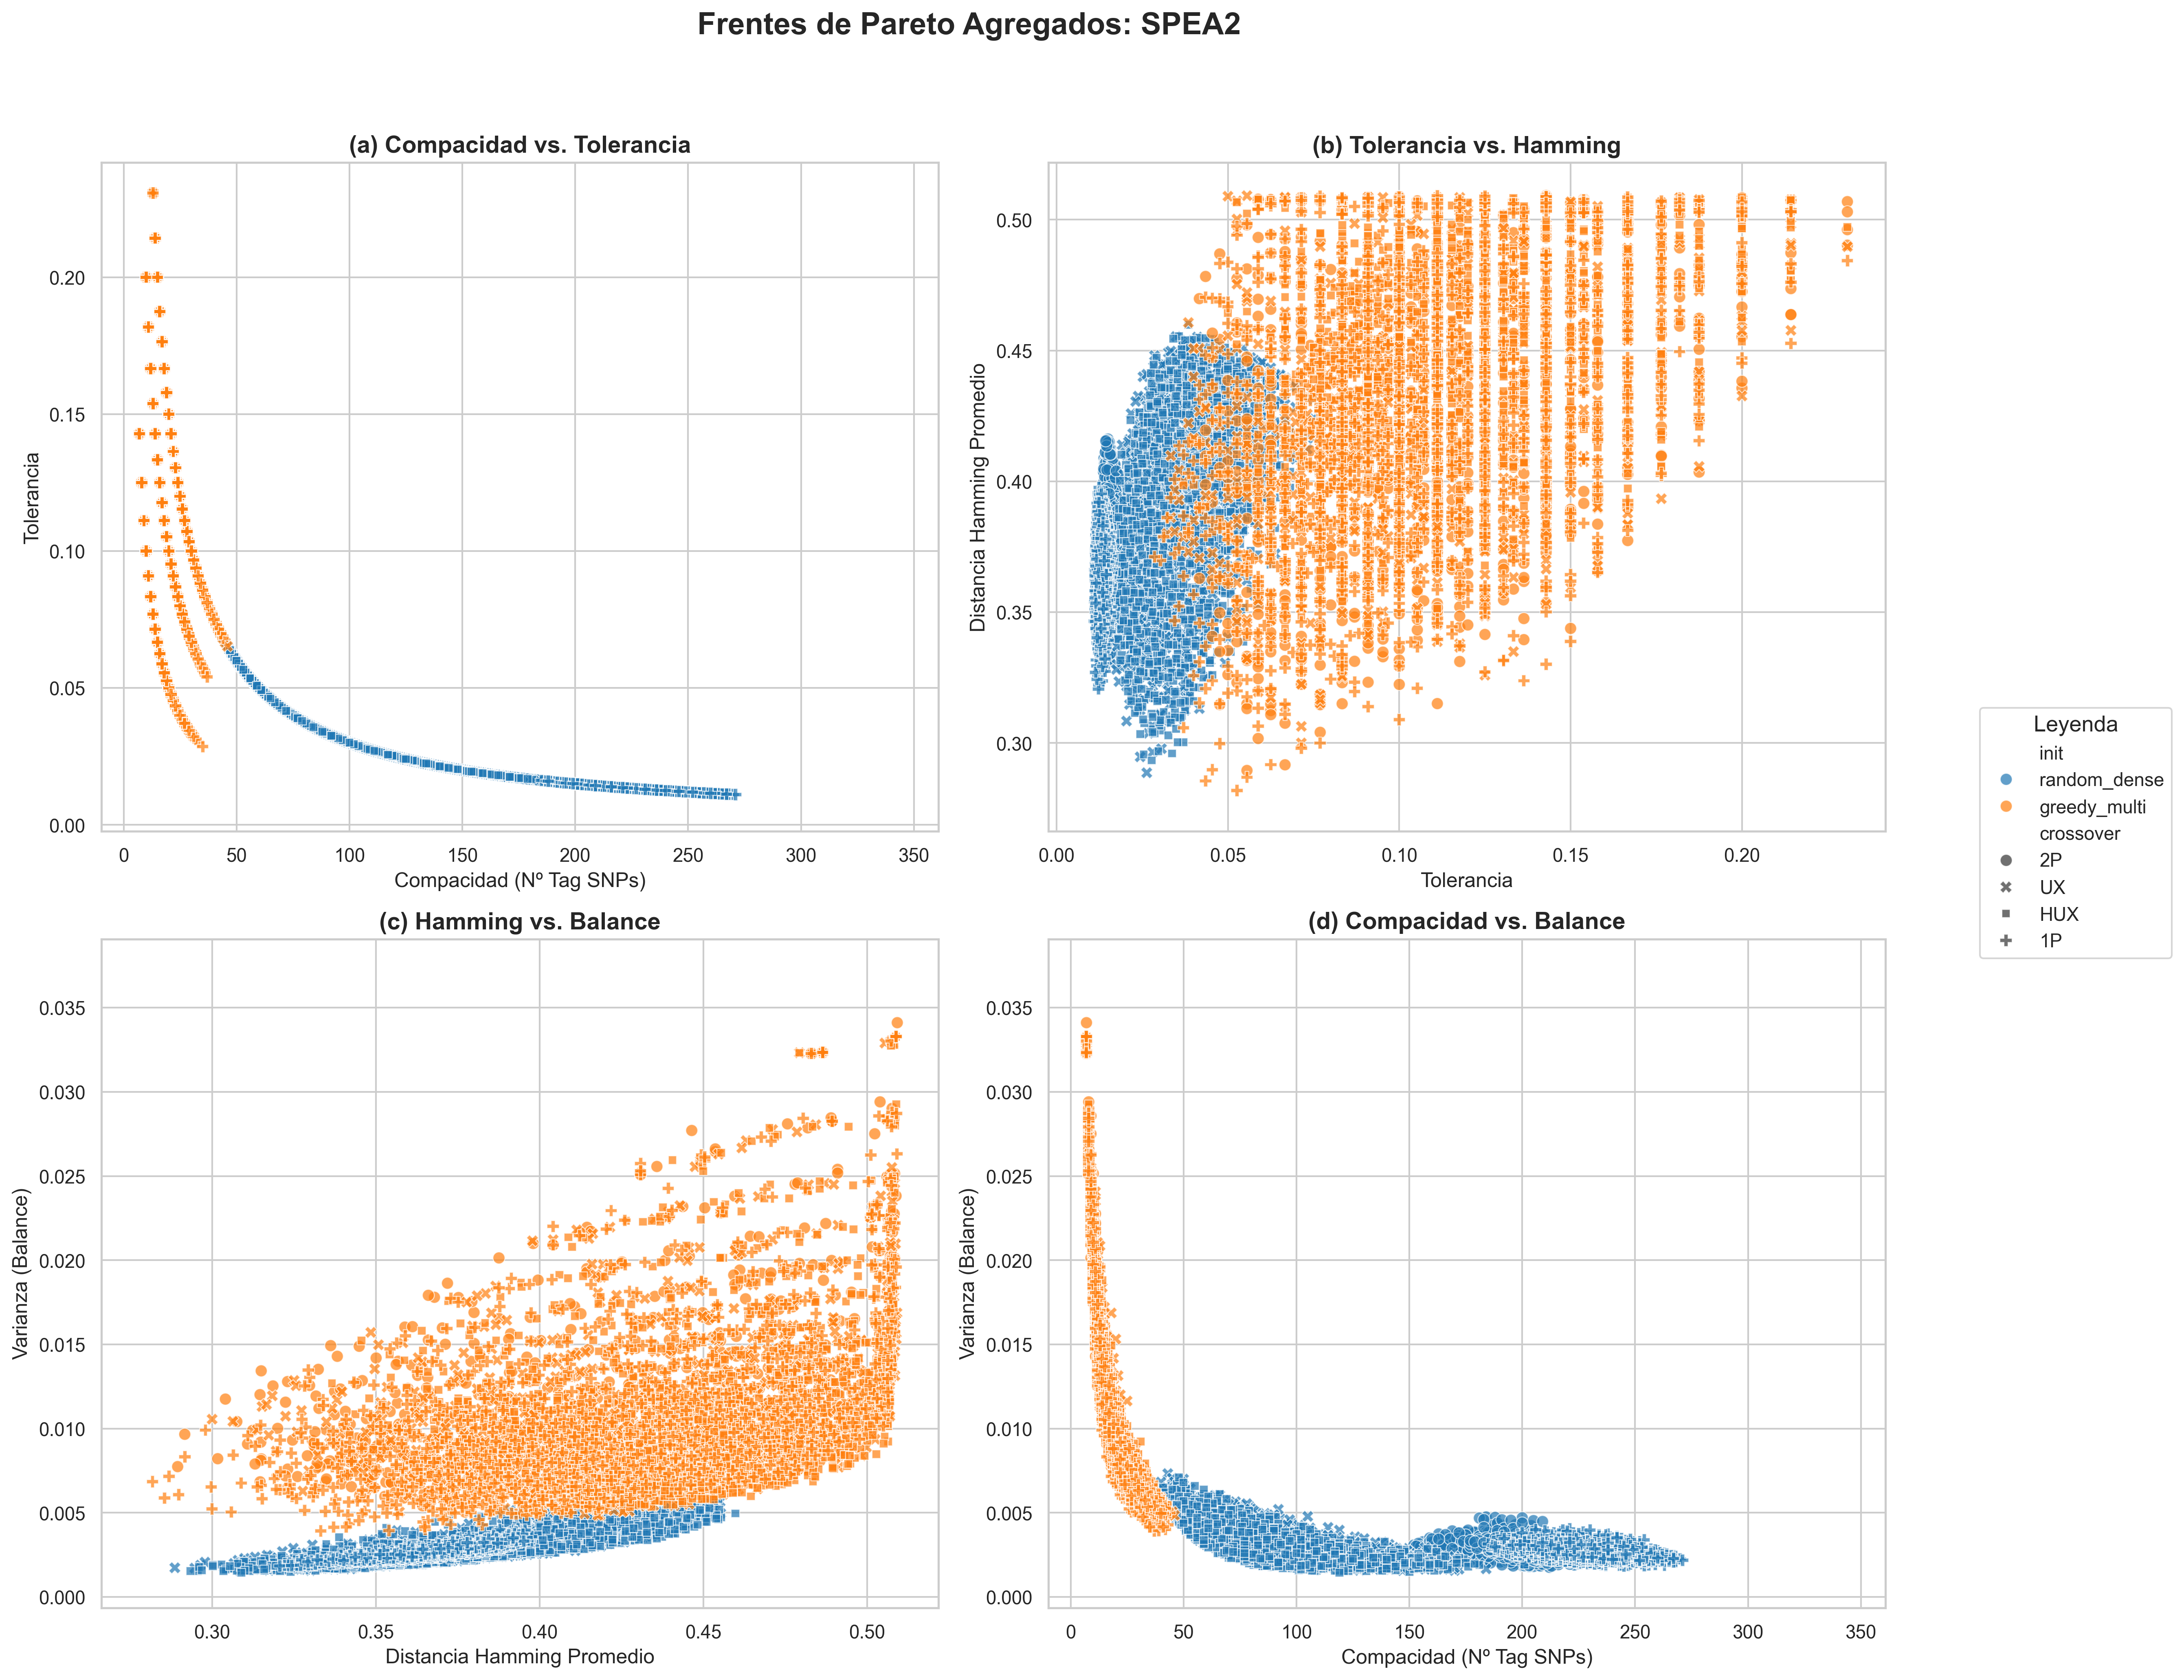
\includegraphics[width=0.22\textwidth]{analisis_assets/frentes_pareto_agregados_spea2_full.png} & 
\includegraphics[width=0.22\textwidth]{analisis_assets/frentes_pareto_agregados_moead_tche_full.png} \\
        NSGA-II & NSGA-III & SPEA2 & MOEA/D \\
        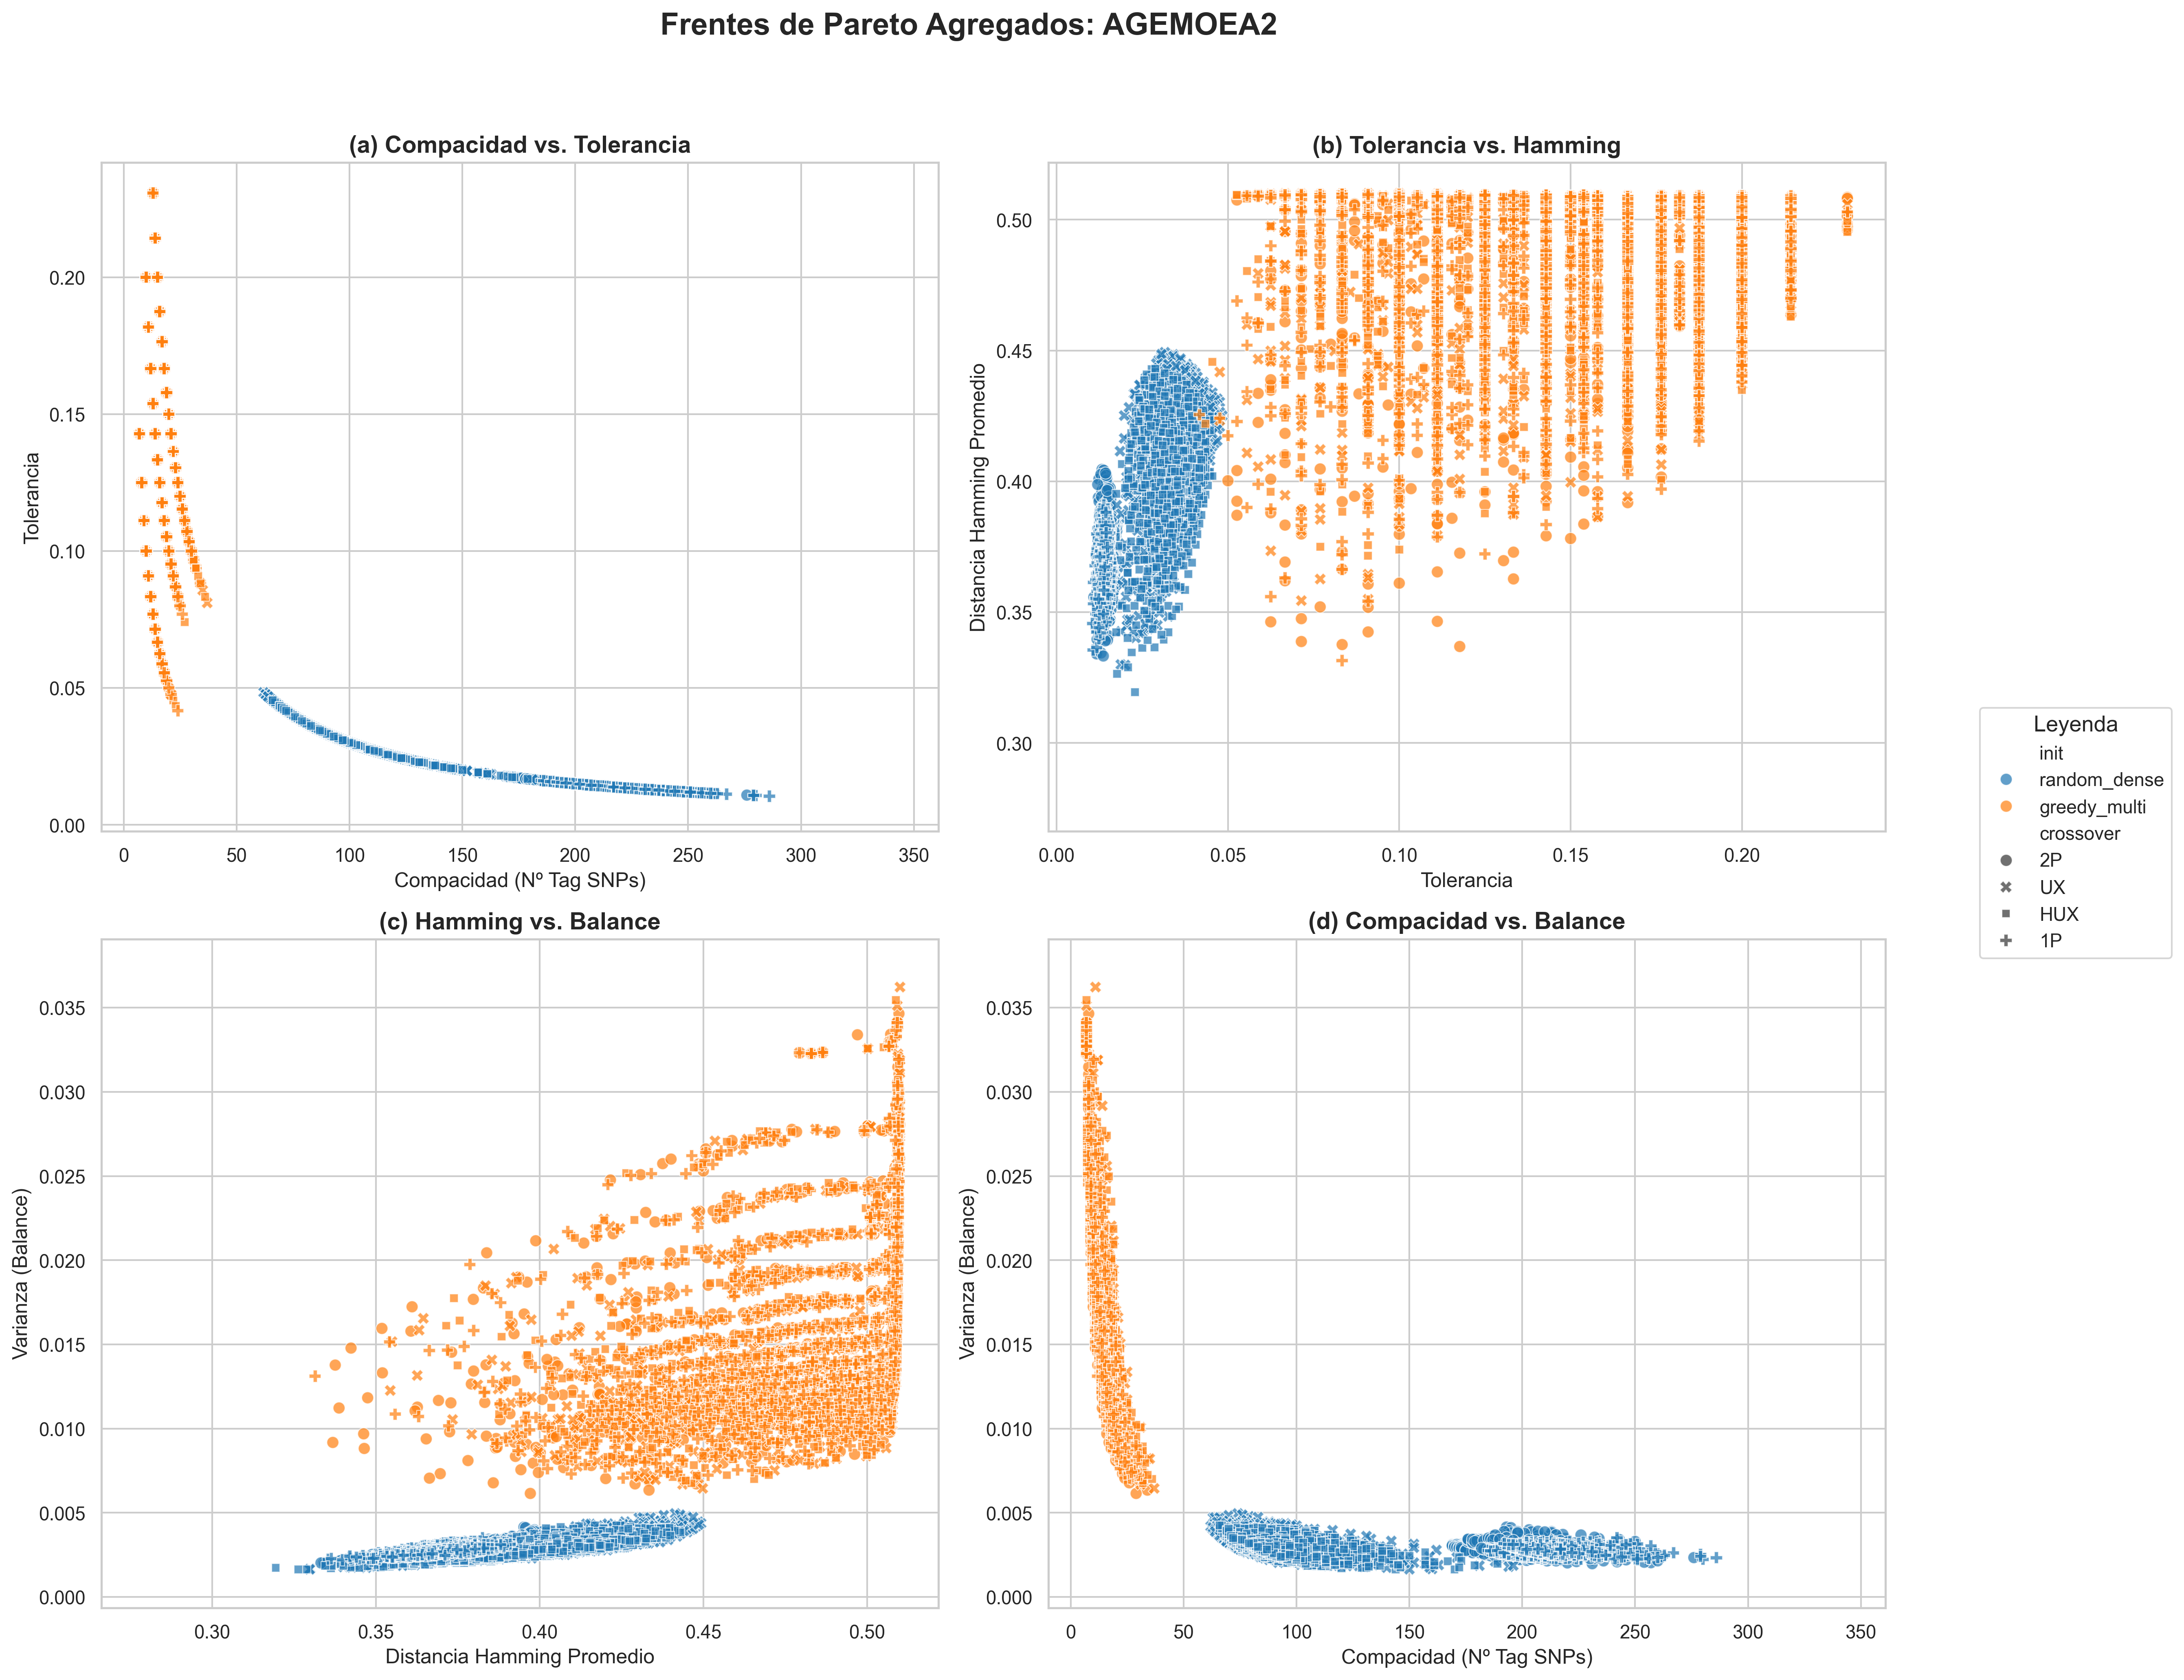
\includegraphics[width=0.22\textwidth]{analisis_assets/frentes_pareto_agregados_agemoea2_full.png} & 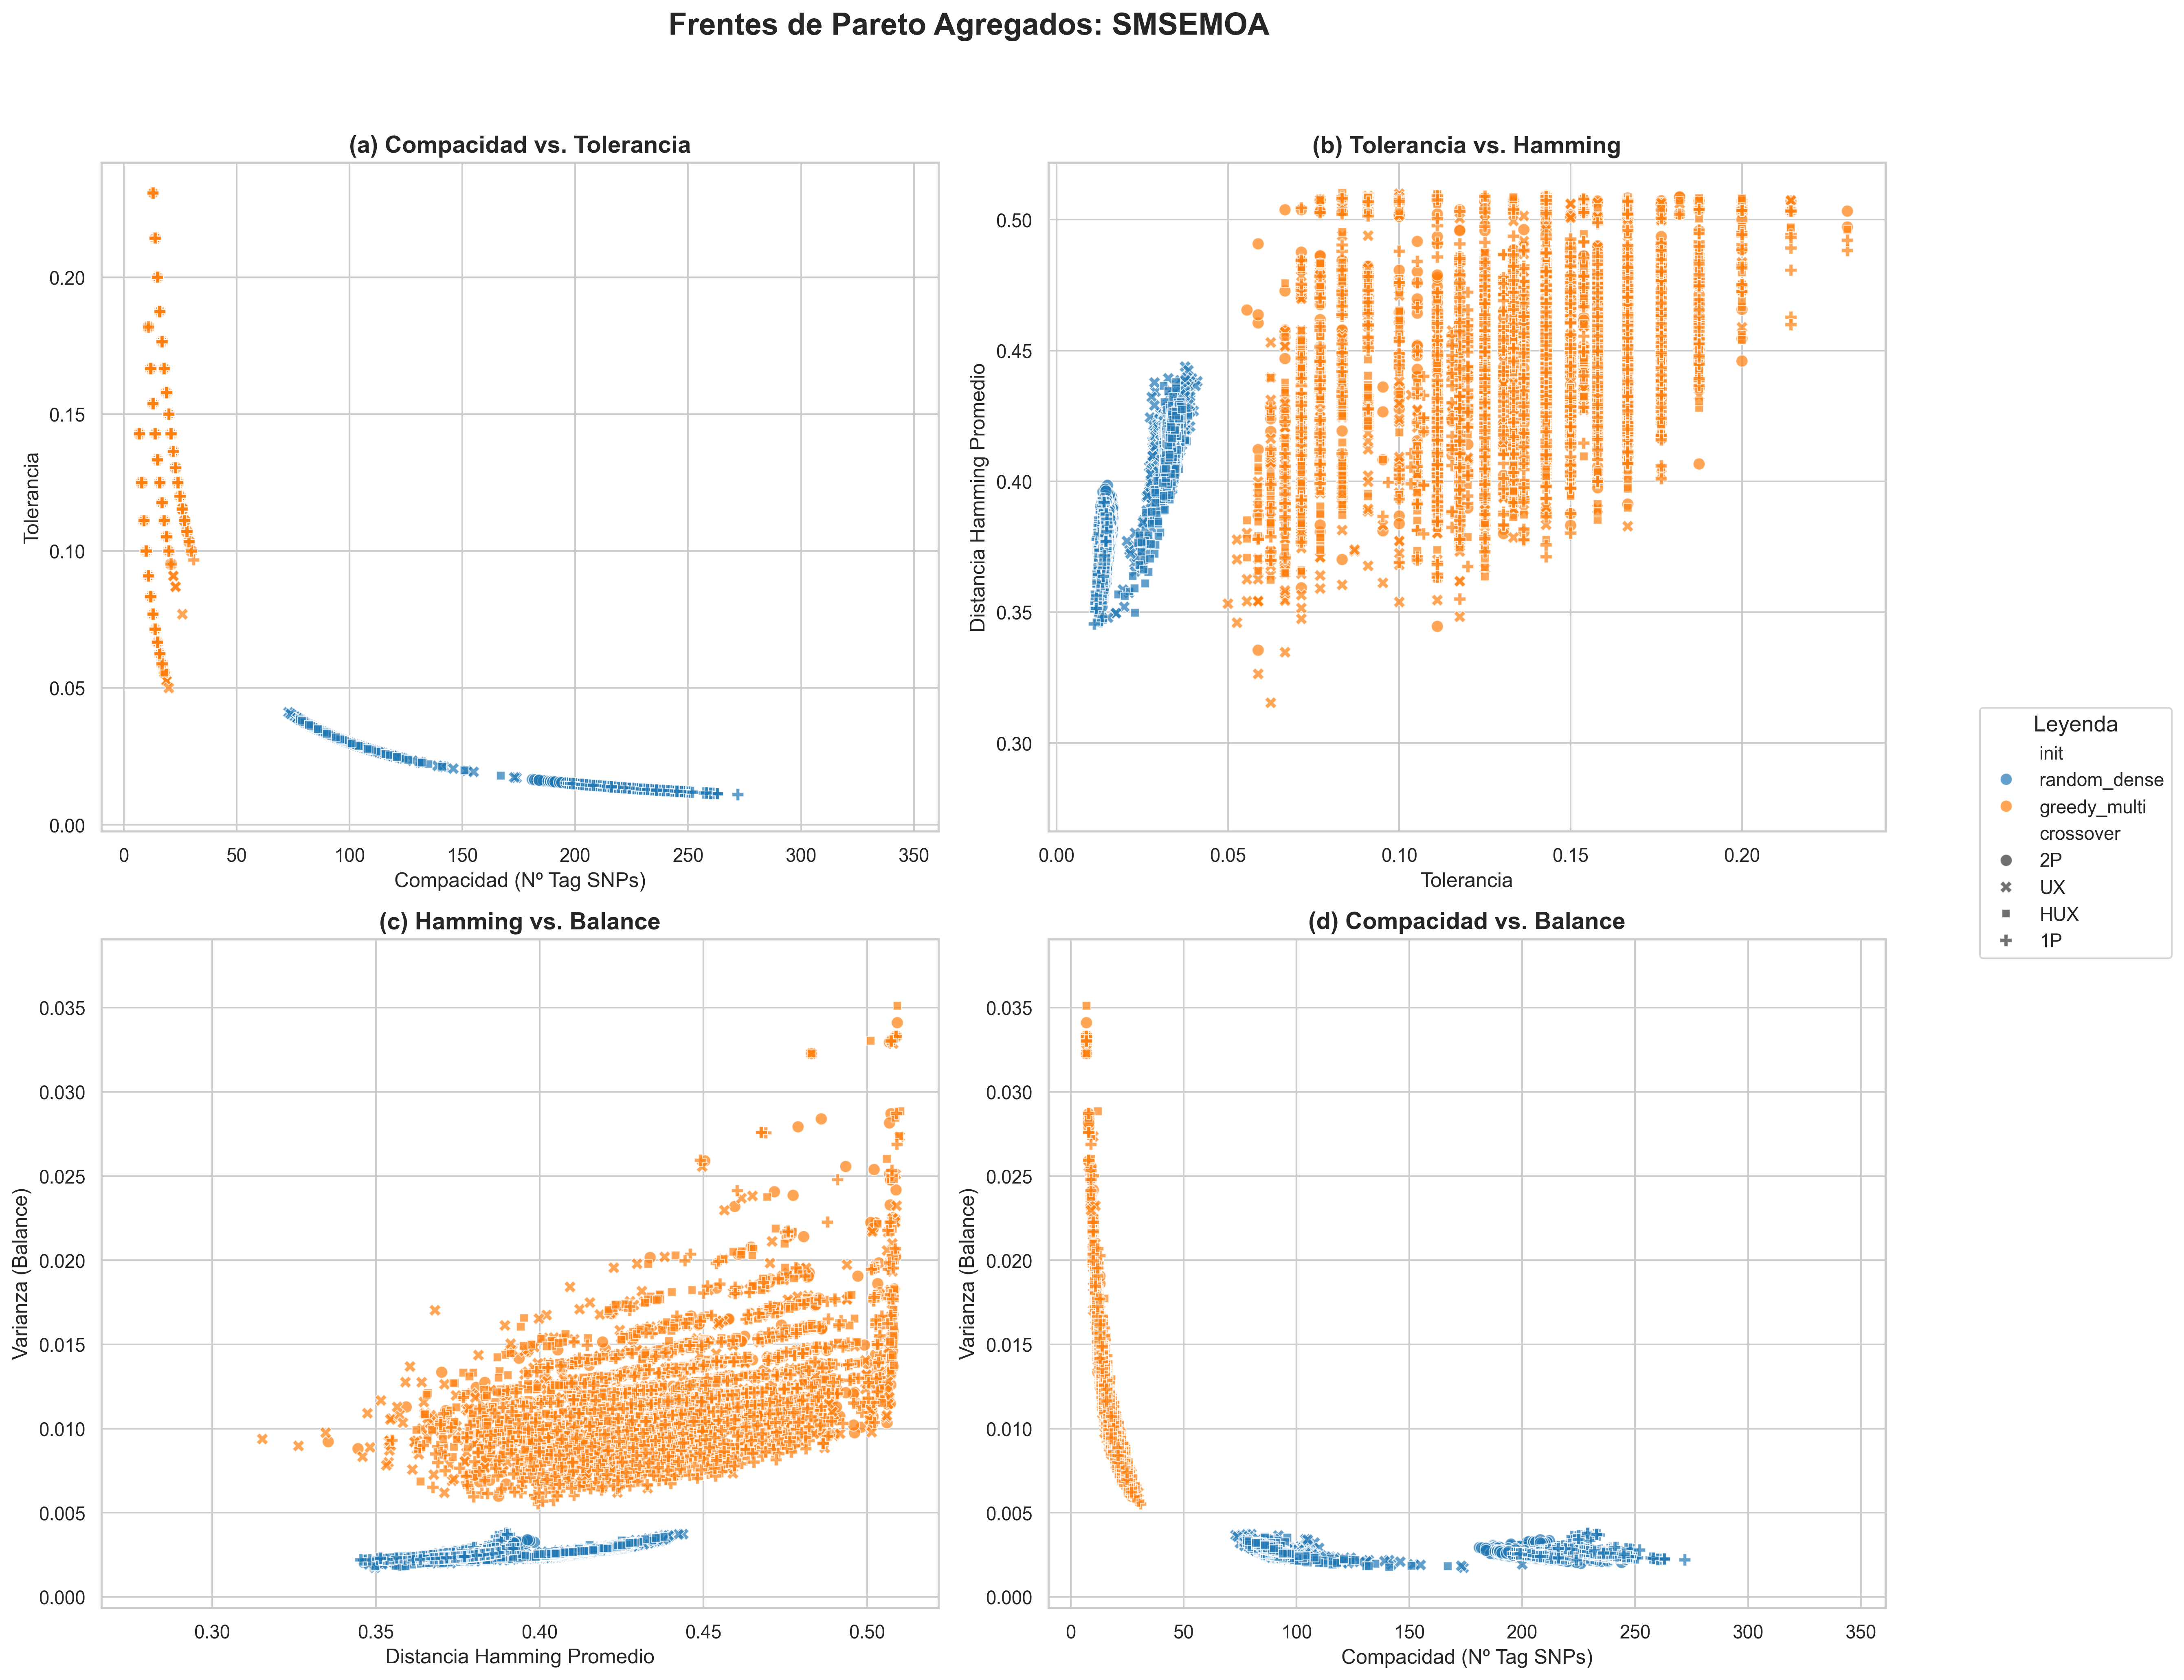
\includegraphics[width=0.22\textwidth]{analisis_assets/frentes_pareto_agregados_smsemoa_full.png} & 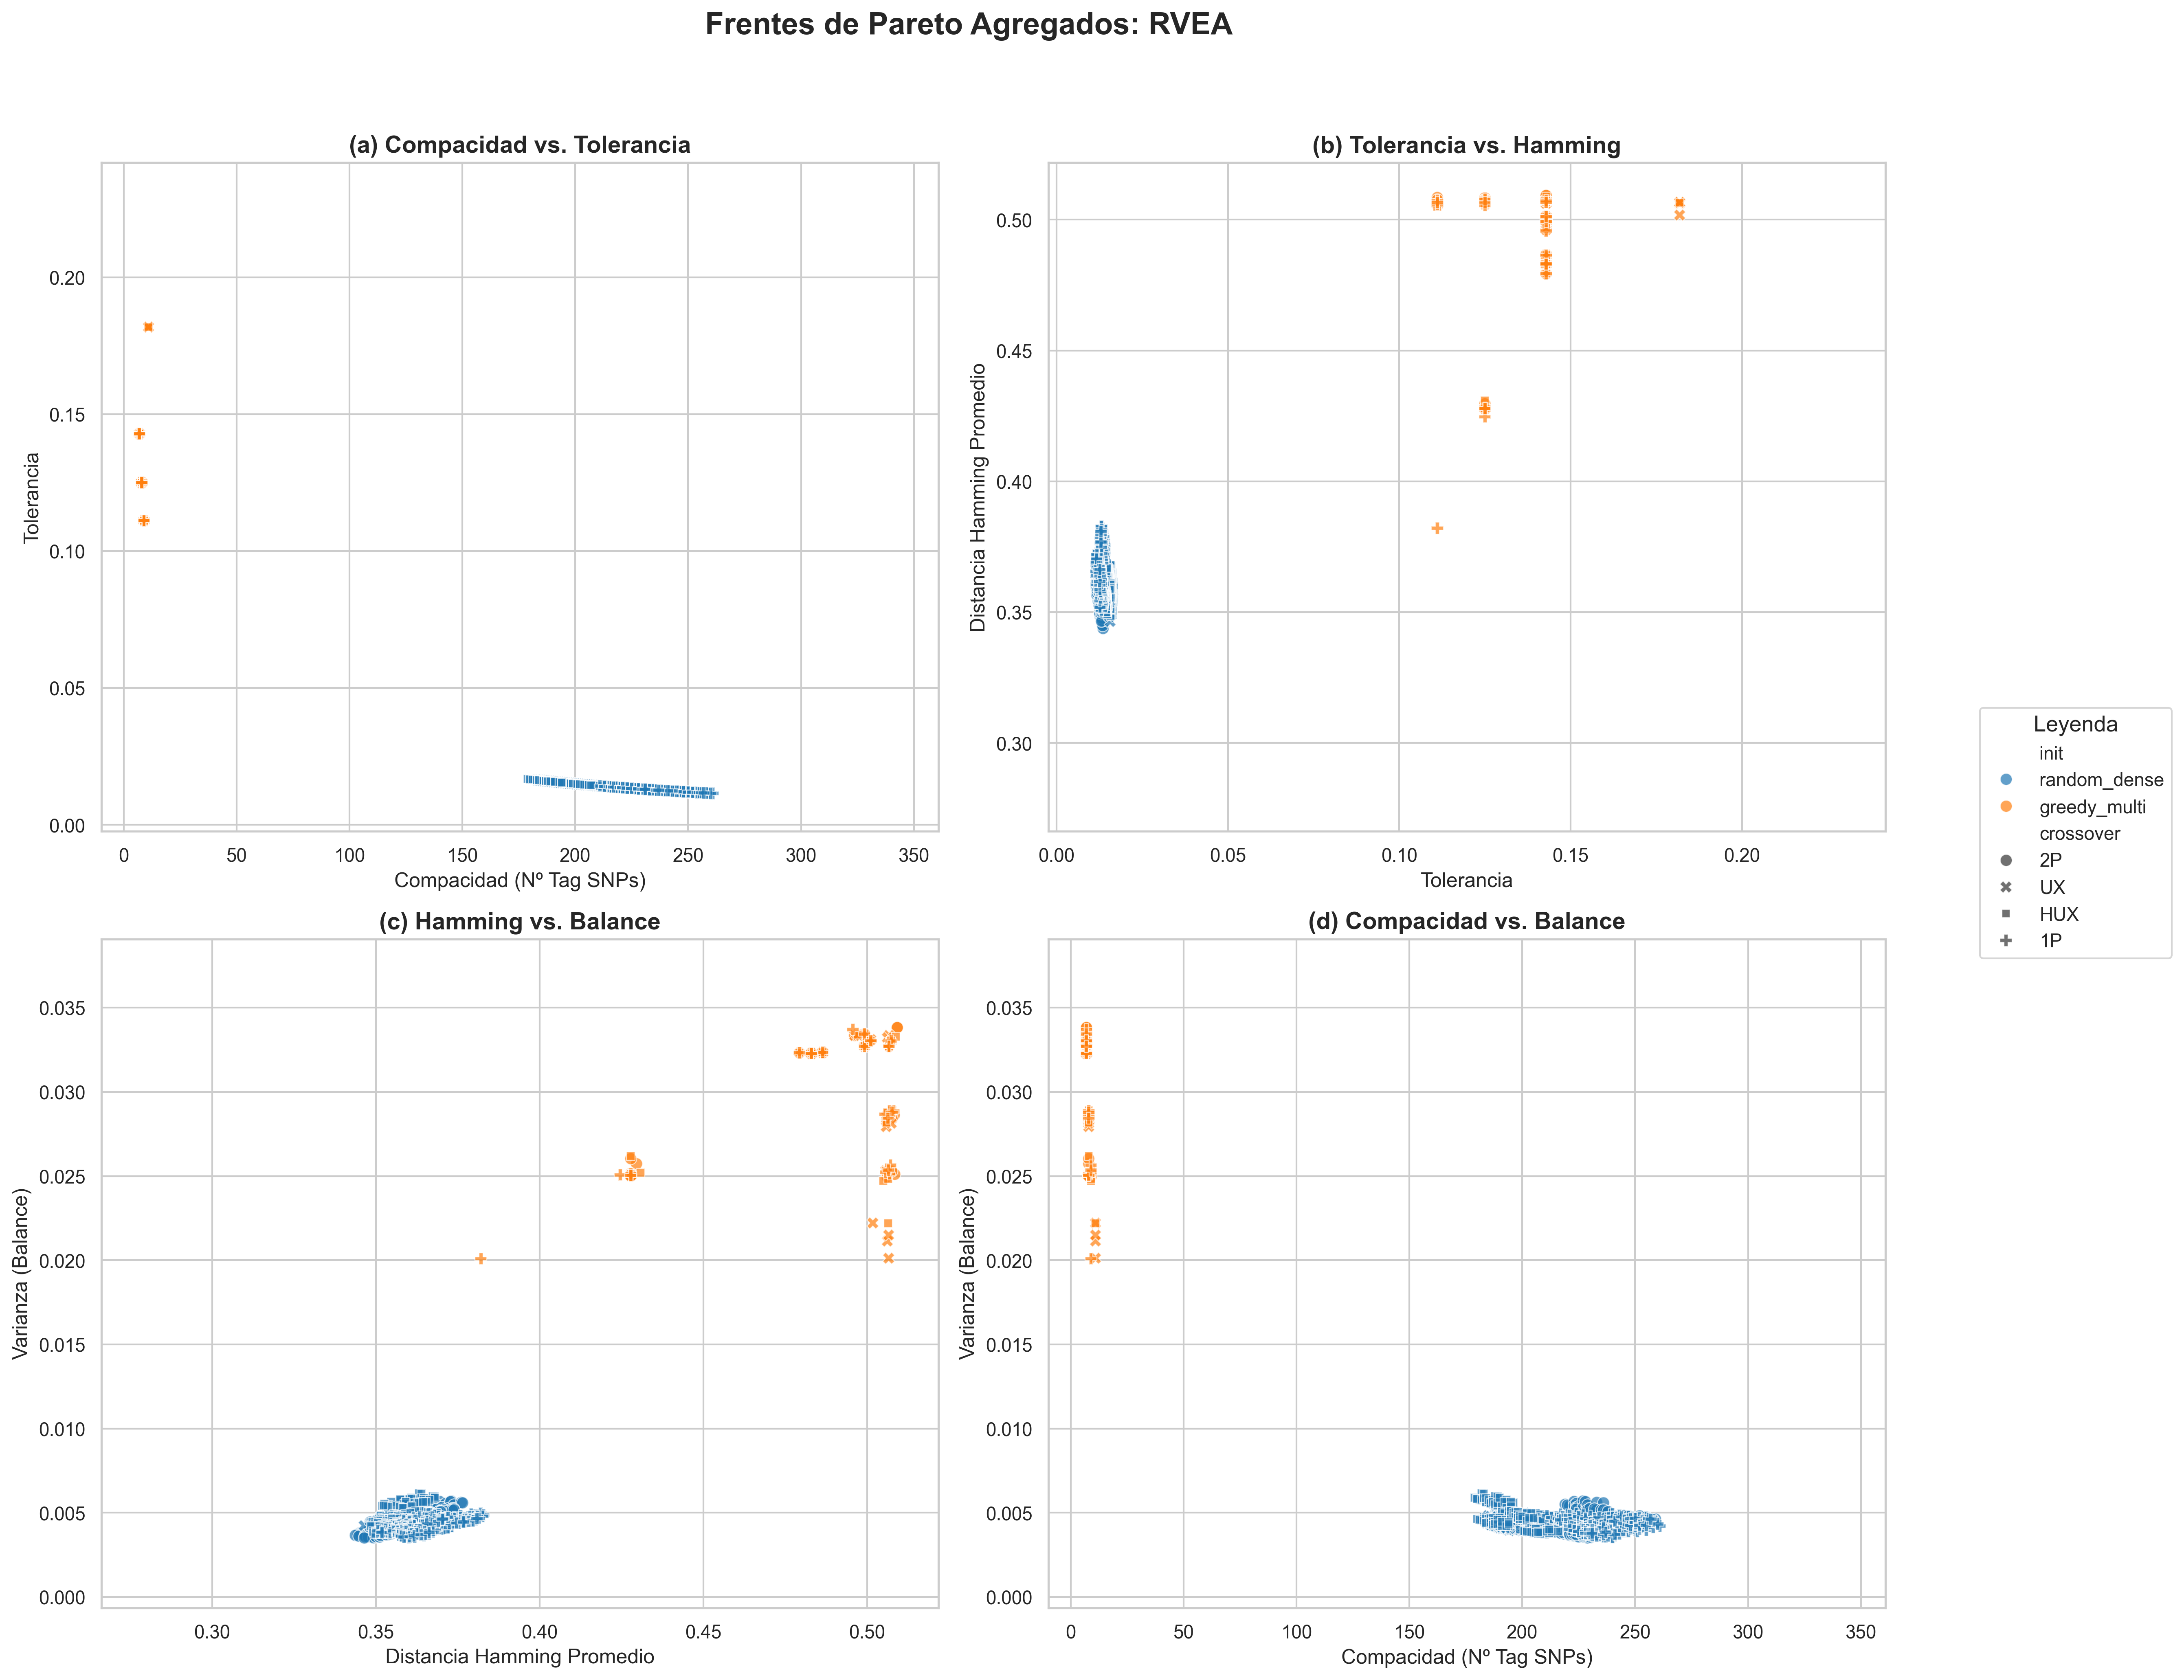
\includegraphics[width=0.22\textwidth]{analisis_assets/frentes_pareto_agregados_rvea_full.png} & 
\includegraphics[width=0.22\textwidth]{analisis_assets/frentes_pareto_global_full.png} \\
        AGE-MOEA2 & SMS-EMOA & RVEA & \textbf{Frente Global} \\
    \end{tabular}
    \caption{Frentes de Pareto agregados por algoritmo y Frente Global consolidado.}
\end{figure}

\section{Análisis de Resultados y Validación Estadística}
A continuación se presentan los rankings detallados (Top 10 Mejores) y su validación estadística mediante el test de Kruskal-Wallis y comparaciones Post-Hoc de Dunn.

\subsection{Range ($\uparrow$)}
\tablaranking{
    1 & SPEA2 (greedy\_multi+2P) & $0.5384 \pm 0.0214$ \\
    2 & NSGA2 (greedy\_multi+HUX) & $0.5357 \pm 0.0297$ \\
    3 & NSGA2 (greedy\_multi+UX) & $0.5356 \pm 0.0128$ \\
    4 & SPEA2 (greedy\_multi+UX) & $0.5279 \pm 0.0121$ \\
    5 & SPEA2 (greedy\_multi+1P) & $0.5244 \pm 0.0345$ \\
    6 & NSGA2 (greedy\_multi+2P) & $0.5232 \pm 0.0502$ \\
    7 & NSGA2 (greedy\_multi+1P) & $0.5192 \pm 0.0147$ \\
    8 & SPEA2 (greedy\_multi+HUX) & $0.4781 \pm 0.0208$ \\
    9 & NSGA3 (greedy\_multi+HUX) & $0.4748 \pm 0.0266$ \\
    10 & AGEMOEA2 (greedy\_multi+2P) & $0.4711 \pm 0.0229$ \\
}{Ranking de la métrica Range (Extensión del frente).}{tab:range}

\textbf{Validación Estadística (Range):}
\begin{itemize}
    \item \textbf{Estadístico H (Kruskal-Wallis):} 248.9606
    \item \textbf{P-valor:} $1.0524 \times 10^{-45}$ (Significativo, $p < 0.05$).
\end{itemize}

\begin{figure}[H]
    \centering
    
\includegraphics[width=0.55\textwidth]{analisis_assets/heatmap_dunn_range_full.png}
    \caption{Post-Hoc Dunn (Range): Significancia de diferencias entre configuraciones.}
\end{figure}

\subsection{MinSum ($\downarrow$)}
\tablaranking{
    1 & SPEA2 (greedy\_multi+2P) & $1.3535 \pm 0.0061$ \\
    2 & AGEMOEA2 (greedy\_multi+HUX) & $1.3538 \pm 0.0038$ \\
    3 & AGEMOEA2 (greedy\_multi+UX) & $1.3539 \pm 0.0049$ \\
    4 & MOEAD\_TCHE (greedy\_multi+UX) & $1.3546 \pm 0.0053$ \\
    5 & AGEMOEA2 (greedy\_multi+2P) & $1.3550 \pm 0.0024$ \\
    6 & AGEMOEA2 (greedy\_multi+1P) & $1.3551 \pm 0.0040$ \\
    7 & NSGA3 (greedy\_multi+HUX) & $1.3557 \pm 0.0029$ \\
    8 & NSGA3 (greedy\_multi+2P) & $1.3563 \pm 0.0009$ \\
    9 & NSGA2 (greedy\_multi+2P) & $1.3564 \pm 0.0116$ \\
    10 & NSGA2 (greedy\_multi+HUX) & $1.3564 \pm 0.0049$ \\
}{Ranking de la métrica MinSum.}{tab:minsum}

\textbf{Validación Estadística (MinSum):}
\begin{itemize}
    \item \textbf{Estadístico H (Kruskal-Wallis):} 246.5203
    \item \textbf{P-valor:} $3.3788 \times 10^{-45}$ (Significativo, $p < 0.05$).
\end{itemize}

\begin{figure}[H]
    \centering
    
\includegraphics[width=0.55\textwidth]{analisis_assets/heatmap_dunn_minsum_full.png}
    \caption{Post-Hoc Dunn (MinSum).}
\end{figure}

\subsection{SumMin ($\downarrow$)}
\tablaranking{
    1 & SPEA2 (greedy\_multi+2P) & $1.2935 \pm 0.0081$ \\
    2 & NSGA2 (greedy\_multi+2P) & $1.2964 \pm 0.0106$ \\
    3 & NSGA2 (greedy\_multi+HUX) & $1.3010 \pm 0.0083$ \\
    4 & AGEMOEA2 (greedy\_multi+2P) & $1.3010 \pm 0.0093$ \\
    5 & AGEMOEA2 (greedy\_multi+UX) & $1.3011 \pm 0.0093$ \\
    6 & SPEA2 (greedy\_multi+1P) & $1.3015 \pm 0.0063$ \\
    7 & SMSEMOA (greedy\_multi+1P) & $1.3028 \pm 0.0086$ \\
    8 & SPEA2 (greedy\_multi+UX) & $1.3029 \pm 0.0065$ \\
    9 & SPEA2 (greedy\_multi+HUX) & $1.3041 \pm 0.0077$ \\
    10 & AGEMOEA2 (greedy\_multi+HUX) & $1.3050 \pm 0.0086$ \\
}{Ranking de la métrica SumMin.}{tab:summin}

\textbf{Validación Estadística (SumMin):}
\begin{itemize}
    \item \textbf{Estadístico H (Kruskal-Wallis):} 247.5870
    \item \textbf{P-valor:} $2.0293 \times 10^{-45}$ (Significativo, $p < 0.05$).
\end{itemize}

\begin{figure}[H]
    \centering
    
\includegraphics[width=0.55\textwidth]{analisis_assets/heatmap_dunn_summin_full.png}
    \caption{Post-Hoc Dunn (SumMin).}
\end{figure}

\subsection{MaxToleranceRate ($\uparrow$)}
\tablaranking{
    1 & AGEMOEA2 (greedy\_multi+1P) & $0.0204 \pm 0.0000$ \\
    2 & AGEMOEA2 (greedy\_multi+2P) & $0.0204 \pm 0.0000$ \\
    3 & AGEMOEA2 (greedy\_multi+HUX) & $0.0204 \pm 0.0000$ \\
    4 & AGEMOEA2 (greedy\_multi+UX) & $0.0204 \pm 0.0000$ \\
    5 & NSGA2 (greedy\_multi+1P) & $0.0204 \pm 0.0000$ \\
    6 & NSGA2 (greedy\_multi+2P) & $0.0204 \pm 0.0000$ \\
    7 & NSGA2 (greedy\_multi+HUX) & $0.0204 \pm 0.0000$ \\
    8 & NSGA2 (greedy\_multi+UX) & $0.0204 \pm 0.0000$ \\
    9 & SMSEMOA (greedy\_multi+1P) & $0.0204 \pm 0.0000$ \\
    10 & SMSEMOA (greedy\_multi+2P) & $0.0204 \pm 0.0000$ \\
}{Ranking de MaxToleranceRate.}{tab:maxtol}

\textbf{Validación Estadística (MaxToleranceRate):}
\begin{itemize}
    \item \textbf{Estadístico H (Kruskal-Wallis):} 254.4421
    \item \textbf{P-valor:} $7.6469 \times 10^{-47}$ (Significativo, $p < 0.05$).
\end{itemize}

\begin{figure}[H]
    \centering
    
\includegraphics[width=0.55\textwidth]{analisis_assets/heatmap_dunn_maxtolerancerate_full.png}
    \caption{Post-Hoc Dunn (MaxToleranceRate).}
\end{figure}

\subsection{AvgToleranceRate ($\uparrow$)}
\tablaranking{
    1 & RVEA (greedy\_multi+UX) & $0.0183 \pm 0.0003$ \\
    2 & RVEA (greedy\_multi+HUX) & $0.0178 \pm 0.0002$ \\
    3 & RVEA (greedy\_multi+2P) & $0.0177 \pm 0.0002$ \\
    4 & RVEA (greedy\_multi+1P) & $0.0175 \pm 0.0002$ \\
    5 & NSGA3 (greedy\_multi+1P) & $0.0105 \pm 0.0003$ \\
    6 & NSGA3 (greedy\_multi+2P) & $0.0105 \pm 0.0003$ \\
    7 & NSGA3 (greedy\_multi+UX) & $0.0104 \pm 0.0003$ \\
    8 & NSGA3 (greedy\_multi+HUX) & $0.0103 \pm 0.0002$ \\
    9 & AGEMOEA2 (greedy\_multi+1P) & $0.0102 \pm 0.0002$ \\
    10 & AGEMOEA2 (greedy\_multi+2P) & $0.0102 \pm 0.0002$ \\
}{Ranking de AvgToleranceRate.}{tab:avgtol}

\textbf{Validación Estadística (AvgToleranceRate):}
\begin{itemize}
    \item \textbf{Estadístico H (Kruskal-Wallis):} 254.7534
    \item \textbf{P-valor:} $6.5885 \times 10^{-47}$ (Significativo, $p < 0.05$).
\end{itemize}

\begin{figure}[H]
    \centering
    
\includegraphics[width=0.55\textwidth]{analisis_assets/heatmap_dunn_avgtolerancerate_full.png}
    \caption{Post-Hoc Dunn (AvgToleranceRate).}
\end{figure}

\subsection{AvgHammingDistance ($\uparrow$)}
\tablaranking{
    1 & RVEA (greedy\_multi+HUX) & $0.4958 \pm 0.0063$ \\
    2 & RVEA (greedy\_multi+UX) & $0.4929 \pm 0.0068$ \\
    3 & MOEAD\_TCHE (greedy\_multi+1P) & $0.4929 \pm 0.0116$ \\
    4 & MOEAD\_TCHE (greedy\_multi+2P) & $0.4903 \pm 0.0057$ \\
    5 & MOEAD\_TCHE (greedy\_multi+HUX) & $0.4889 \pm 0.0044$ \\
    6 & RVEA (greedy\_multi+2P) & $0.4885 \pm 0.0006$ \\
    7 & RVEA (greedy\_multi+1P) & $0.4854 \pm 0.0065$ \\
    8 & MOEAD\_TCHE (greedy\_multi+UX) & $0.4847 \pm 0.0038$ \\
    9 & AGEMOEA2 (greedy\_multi+HUX) & $0.4826 \pm 0.0111$ \\
    10 & AGEMOEA2 (greedy\_multi+UX) & $0.4808 \pm 0.0016$ \\
}{Ranking de Diversidad Biológica (Hamming).}{tab:hamming}

\textbf{Validación Estadística (AvgHammingDistance):}
\begin{itemize}
    \item \textbf{Estadístico H (Kruskal-Wallis):} 257.4241
    \item \textbf{P-valor:} $1.8347 \times 10^{-47}$ (Significativo, $p < 0.05$).
\end{itemize}

\begin{figure}[H]
    \centering
    
\includegraphics[width=0.55\textwidth]{analisis_assets/heatmap_dunn_avghammingdistance_full.png}
    \caption{Post-Hoc Dunn (AvgHammingDistance).}
\end{figure}

\subsection{Hypervolume ($\uparrow$)}
\tablaranking{
    1 & SPEA2 (greedy\_multi+2P) & $0.2319 \pm 0.0051$ \\
    2 & NSGA2 (greedy\_multi+2P) & $0.2295 \pm 0.0065$ \\
    3 & AGEMOEA2 (greedy\_multi+UX) & $0.2295 \pm 0.0061$ \\
    4 & AGEMOEA2 (greedy\_multi+2P) & $0.2295 \pm 0.0060$ \\
    5 & NSGA3 (greedy\_multi+2P) & $0.2288 \pm 0.0062$ \\
    6 & MOEAD\_TCHE (greedy\_multi+UX) & $0.2283 \pm 0.0063$ \\
    7 & AGEMOEA2 (greedy\_multi+HUX) & $0.2273 \pm 0.0060$ \\
    8 & MOEAD\_TCHE (greedy\_multi+1P) & $0.2273 \pm 0.0055$ \\
    9 & NSGA3 (greedy\_multi+HUX) & $0.2267 \pm 0.0064$ \\
    10 & SMSEMOA (greedy\_multi+2P) & $0.2265 \pm 0.0060$ \\
}{Ranking de Hypervolume.}{tab:hv}

\textbf{Validación Estadística (Hypervolume):}
\begin{itemize}
    \item \textbf{Estadístico H (Kruskal-Wallis):} 247.0778
    \item \textbf{P-valor:} $2.5885 \times 10^{-45}$ (Significativo, $p < 0.05$).
\end{itemize}

\begin{figure}[H]
    \centering
    
\includegraphics[width=0.55\textwidth]{analisis_assets/heatmap_dunn_hypervolume_full.png}
    \caption{Post-Hoc Dunn (Hypervolume).}
\end{figure}

\subsection{IGD+ ($\downarrow$)}
\tablaranking{
    1 & NSGA2 (greedy\_multi+HUX) & $0.0010 \pm 0.0009$ \\
    2 & NSGA2 (greedy\_multi+1P) & $0.0013 \pm 0.0007$ \\
    3 & NSGA2 (greedy\_multi+2P) & $0.0013 \pm 0.0007$ \\
    4 & AGEMOEA2 (greedy\_multi+HUX) & $0.0023 \pm 0.0034$ \\
    5 & NSGA2 (greedy\_multi+UX) & $0.0023 \pm 0.0034$ \\
    6 & AGEMOEA2 (greedy\_multi+UX) & $0.0038 \pm 0.0036$ \\
    7 & AGEMOEA2 (greedy\_multi+1P) & $0.0044 \pm 0.0047$ \\
    8 & RVEA (greedy\_multi+2P) & $0.0055 \pm 0.0051$ \\
    9 & SPEA2 (greedy\_multi+HUX) & $0.0055 \pm 0.0028$ \\
    10 & SMSEMOA (greedy\_multi+1P) & $0.0056 \pm 0.0036$ \\
}{Ranking de IGD+.}{tab:igd}

\textbf{Validación Estadística (IGD+):}
\begin{itemize}
    \item \textbf{Estadístico H (Kruskal-Wallis):} 245.7910
    \item \textbf{P-valor:} $4.7874 \times 10^{-45}$ (Significativo, $p < 0.05$).
\end{itemize}

\begin{figure}[H]
    \centering
    
\includegraphics[width=0.55\textwidth]{analisis_assets/heatmap_dunn_igd+_full.png}
    \caption{Post-Hoc Dunn (IGD+).}
\end{figure}

\subsection{GD+ ($\downarrow$)}
\tablaranking{
    1 & RVEA (greedy\_multi+UX) & $0.0889 \pm 0.0231$ \\
    2 & RVEA (greedy\_multi+HUX) & $0.0915 \pm 0.0214$ \\
    3 & MOEAD\_TCHE (greedy\_multi+1P) & $0.1096 \pm 0.0433$ \\
    4 & MOEAD\_TCHE (greedy\_multi+2P) & $0.1163 \pm 0.0270$ \\
    5 & RVEA (greedy\_multi+2P) & $0.1223 \pm 0.0020$ \\
    6 & MOEAD\_TCHE (greedy\_multi+HUX) & $0.1229 \pm 0.0190$ \\
    7 & RVEA (greedy\_multi+1P) & $0.1358 \pm 0.0260$ \\
    8 & MOEAD\_TCHE (greedy\_multi+UX) & $0.1401 \pm 0.0108$ \\
    9 & AGEMOEA2 (greedy\_multi+HUX) & $0.1695 \pm 0.0065$ \\
    10 & AGEMOEA2 (greedy\_multi+1P) & $0.1782 \pm 0.0203$ \\
}{Ranking de GD+.}{tab:gd}

\textbf{Validación Estadística (GD+):}
\begin{itemize}
    \item \textbf{Estadístico H (Kruskal-Wallis):} 257.2160
    \item \textbf{P-valor:} $2.0269 \times 10^{-47}$ (Significativo, $p < 0.05$).
\end{itemize}

\begin{figure}[H]
    \centering
    
\includegraphics[width=0.55\textwidth]{analisis_assets/heatmap_dunn_gd+_full.png}
    \caption{Post-Hoc Dunn (GD+).}
\end{figure}

\sectionbreak

\subsection{Ranking Promedio Global ($\downarrow$)}
Este ranking consolida el desempeño de cada configuración en las 9 métricas anteriores.

\tablaranking{
    1 & AGEMOEA2 (greedy\_multi+UX) & $8.1667 \pm 0.0000$ \\
    2 & AGEMOEA2 (greedy\_multi+HUX) & $8.7778 \pm 0.0000$ \\
    3 & AGEMOEA2 (greedy\_multi+2P) & $9.0556 \pm 0.0000$ \\
    4 & NSGA2 (greedy\_multi+2P) & $10.5556 \pm 0.0000$ \\
    5 & AGEMOEA2 (greedy\_multi+1P) & $11.5000 \pm 0.0000$ \\
    6 & NSGA3 (greedy\_multi+2P) & $11.6667 \pm 0.0000$ \\
    7 & NSGA3 (greedy\_multi+HUX) & $11.7222 \pm 0.0000$ \\
    8 & NSGA2 (greedy\_multi+HUX) & $12.5000 \pm 0.0000$ \\
    9 & SPEA2 (greedy\_multi+2P) & $12.8889 \pm 0.0000$ \\
    10 & NSGA3 (greedy\_multi+1P) & $13.6111 \pm 0.0000$ \\
}{Ranking Promedio Global (Friedman: 99.7222, $p < 0.05$).}{tab:overall}

\begin{figure}[H]
    \centering
    
\includegraphics[width=0.7\textwidth]{analisis_assets/heatmap_nemenyi_full.png}
    \caption{Heatmap de Significancia Nemenyi para todas las configuraciones.}
\end{figure}

\subsection{Rankings Promedio por Categoría}

\begin{table}[H]
    \centering
    \begin{subtable}[h]{0.48\textwidth}
        \centering
        \begin{tabular}{rlc}
            \toprule
            Pos. & Algoritmo & Rango \\
            \midrule
            1 & NSGA3 & 2.0000 \\
            2 & AGEMOEA2 & 3.1111 \\
            3 & SPEA2 & 3.1111 \\
            4 & NSGA2 & 4.0000 \\
            5 & SMSEMOA & 4.8889 \\
            6 & RVEA & 5.3333 \\
            7 & MOEAD\_TCHE & 5.5556 \\
            \bottomrule
        \end{tabular}
        \caption{Algoritmo}
    \end{subtable}
    \hfill
    \begin{subtable}[h]{0.48\textwidth}
        \centering
        \begin{tabular}{rlc}
            \toprule
            Pos. & Cruce & Rango \\
            \midrule
            1 & UX & 1.5556 \\
            2 & HUX & 1.5556 \\
            3 & 2P & 2.8889 \\
            4 & 1P & 4.0000 \\
            \bottomrule
        \end{tabular}
        \caption{Operador de Cruce}
    \end{subtable}
    \caption{Rankings Promedio por Algoritmo y Cruce.}
\end{table}

\begin{figure}[H]
    \centering
    \begin{subfigure}[b]{0.45\textwidth}
        
\includegraphics[width=\textwidth]{analisis_assets/heatmap_nemenyi_algorithm_full.png}
        \caption{Significancia por Algoritmo}
    \end{subfigure}
    \hfill
    \begin{subfigure}[b]{0.45\textwidth}
        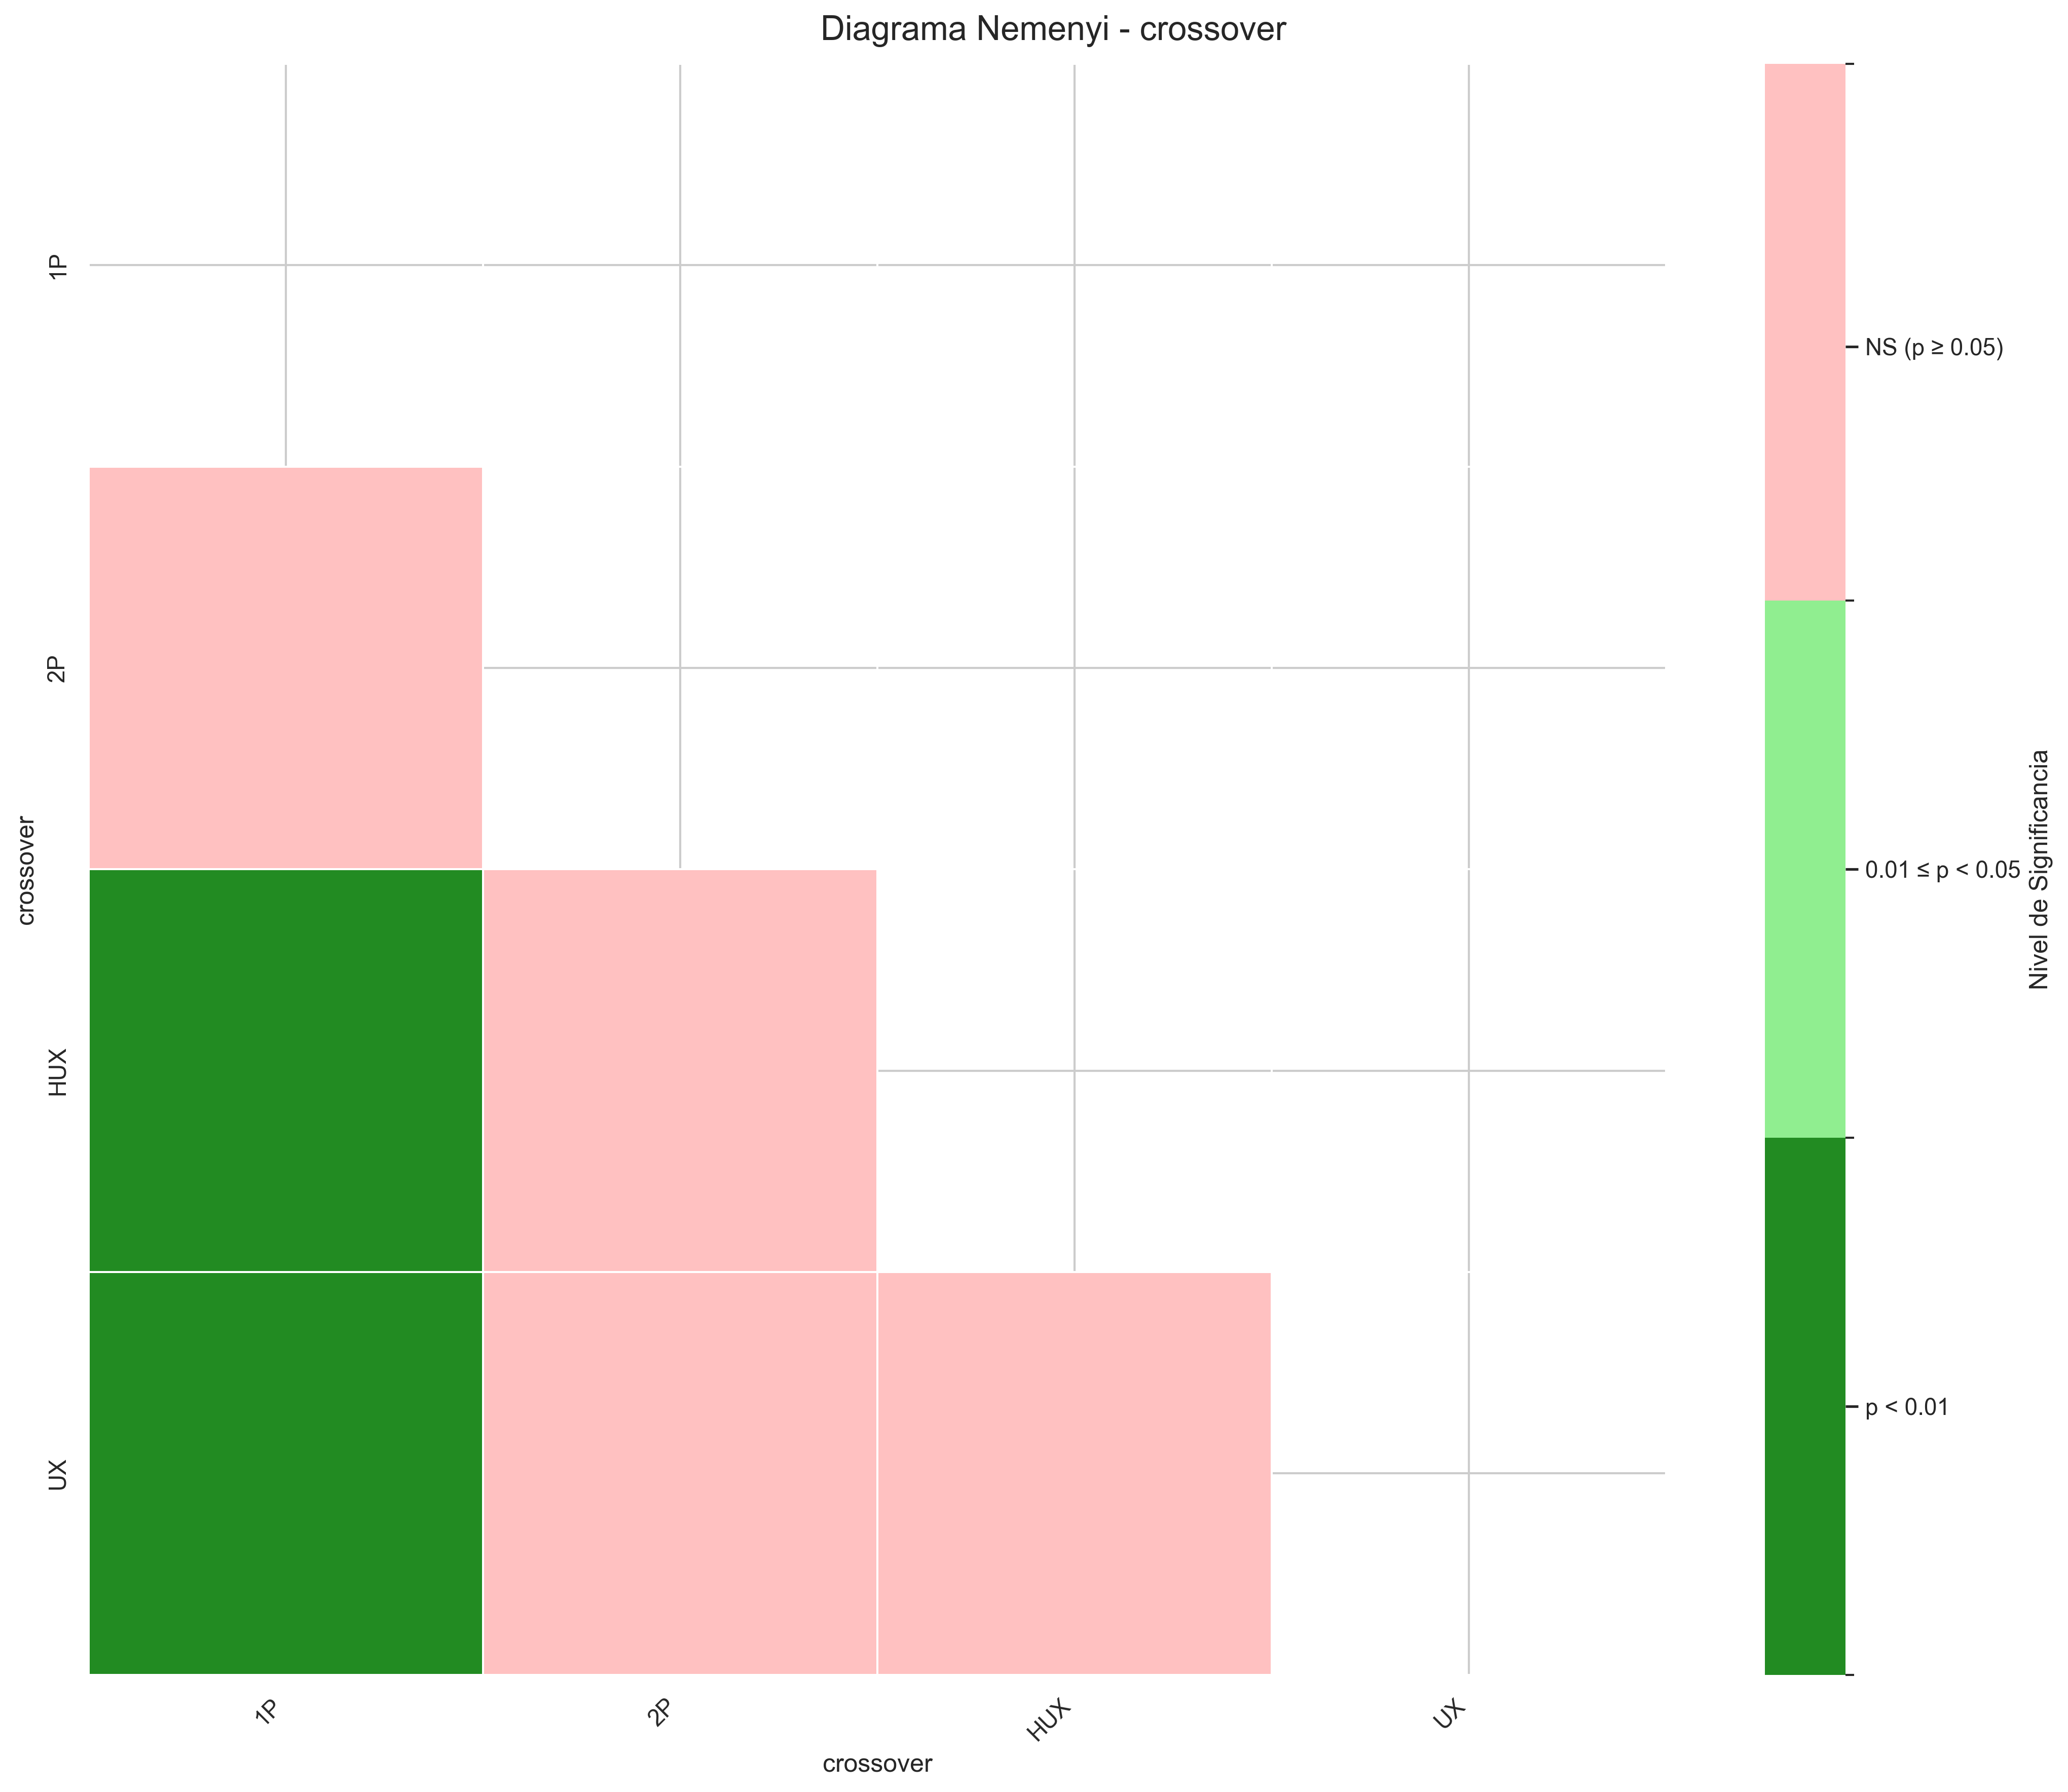
\includegraphics[width=\textwidth]{analisis_assets/heatmap_nemenyi_crossover_full.png}
        \caption{Significancia por Cruce}
    \end{subfigure}
    \caption{Heatmaps de Nemenyi por categoría.}
\end{figure}

\section{Análisis de Resultados}

Con base en las posiciones obtenidas en los rankings estadísticos detallados previamente, se extraen las siguientes conclusiones fundamentales sobre el desempeño de los componentes del motor evolutivo:

\subsection{Mejor Estrategia de Inicialización}
La estrategia \texttt{greedy\_multi} demuestra una superioridad absoluta frente a la aproximación aleatoria. Al analizar el Ranking Promedio Global, se observa que las configuraciones basadas en \texttt{greedy\_multi} monopolizan íntegramente el Top 10, relegando a \texttt{random\_dense} a las posiciones más bajas en la inmensa mayoría de las métricas. Esta profunda polarización en los rankings confirma empíricamente que inyectar conocimiento heurístico biológico en la población inicial es una decisión crítica y determinante para la convergencia en este espacio de búsqueda.

\subsection{Mejor Motor Evolutivo (Algoritmo)}
Atendiendo al Ranking Promedio por Algoritmo, \textbf{NSGA-III} y \textbf{AGE-MOEA-II} se erigen como las opciones más robustas y eficaces. NSGA-III logra la primera posición absoluta (rango 2.0), evidenciando una excelente capacidad estructural para gestionar simultáneamente los múltiples objetivos biológicos. Por su parte, AGE-MOEA-II (rango 3.1) no solo empata en la segunda posición categórica con SPEA2, sino que demuestra una dominancia excepcional al ocupar los tres primeros puestos absolutos en el Ranking Promedio Global. Estos algoritmos han demostrado ser estadísticamente muy superiores a enfoques basados en vectores de referencia estáticos como RVEA o en descomposición como MOEA/D-TCHE, los cuales caen a las últimas posiciones de la tabla.

\subsection{Mejor Operador de Cruce}
El análisis de los rankings por operador revela una clara ventaja de los cruces uniformes sobre los cruces tradicionales. Los operadores \textbf{UX} (Cruce Uniforme) y \textbf{HUX} (Cruce Medio Uniforme) empatan en la primera posición del Ranking Promedio por Cruce (rango 1.55). Esta posición privilegiada contrasta marcadamente con los resultados inferiores del cruce de dos puntos (2P) y el cruce de un punto (1P), que quedan relegados a las posiciones tercera y cuarta respectivamente. Su predominio en los rankings sugiere que una recombinación genética fina (gen a gen) es fundamental para explorar eficazmente cromosomas de alta dimensionalidad.

\sectionbreak

\section{Multi-Criteria Decision Making (MCDM)}
\subsection{Propuestas de Solución}
\begin{itemize}
    \item \textbf{Compromiso (ASF)}: \texttt{SMSEMOA (greedy\_multi)}. Compacidad=17, Tolerancia=0.18.
    \item \textbf{Mejor Knee Point}: \texttt{AGEMOEA2 (greedy\_multi)}.
\end{itemize}

\begin{figure}[H]
    \centering
    
\includegraphics[width=0.7\textwidth]{analisis_assets/mcdm_radar_objetivos_agregado_full.png}
    \caption{Radar de Objetivos MCDM (Agregado).}
\end{figure}

\end{document}
